\documentclass{letter}

\usepackage[left=0.75in, right=0.75in, top=1.1in, bottom=0.75in]{geometry}
\usepackage{fancyhdr, amsmath, amssymb, mathtools, xcolor, graphicx, listings, matlab-prettifier, mathpazo}
\graphicspath{{.}}

\pagestyle{fancy}
\fancyhf{}
\rhead{Page \thepage}
\chead{AMSC808N Homework 2}
\lhead{Tyler Hoffman}
\setlength{\headsep}{0.2in}

\newcounter{problem}
\newcounter{subproblem}[problem]
\newcounter{solution}

\renewcommand{\thesubproblem}{(\alph{subproblem})}

\newcommand{\Problem}[2]{%
	\stepcounter{problem}%
	\leftskip=0pt%
	\theproblem.~\textbf{{#1.}} #2 \par%
}

\newcommand{\Subproblem}[1]{%
	\stepcounter{subproblem}%
	\leftskip=15pt%
	\thesubproblem~ #1 \par%
}

\newcommand{\Solution}[1]{%
	\textbf{Solution.} #1 \par%
}

\newcommand{\Due}[1]{\textbf{Due: #1} \par}

\newcommand{\UNFINISHED}{\textbf{\color{red} UNFINISHED}}
\newcommand{\CHECK}{\textbf{\color{orange} CHECK ME}}

\newcommand{\iu}{{i\mkern1mu}}
\newcommand{\T}{\intercal}
\newcommand{\R}{\mathbb{R}}

\DeclareMathOperator{\diag}{diag}

\lstset{style=Matlab-editor}
\usepackage{hyperref}
\begin{document}
    \Due{24 Sept 2020}
    \Problem{Positive-definite}{Is the matrix $D = (yy^\T) \odot (XX^\T)$ positive-definite? Either prove this statement or give a counterexample.}
    \Solution{First, note the diagonal entries of $XX^\T$ are $x_i^\T x_i = \|x_i\|^2$. Let $x_1 = 0$ and set all the other $x_i = (0, \dots, 1, \dots, 0)^\T$ where the 1 is in the $i$th position. Then the first row and column of $XX^\T$ are all zeros, all the other diagonal entries are 1, and the rest of the matrix is 0. When entrywise multiplied by $yy^\T$ (which is a symmetric matrix of all $\pm 1$), the only entries that remain from $yy^\T$ are on the diagonal. Hence the remaining matrix is a diagonal matrix with a zero in the first diagonal spot and the rest of the diagonal entries are $\pm 1$. Since the matrix is diagonal, the diagonal are its eigenvalues. The matrix here has a zero eigenvalue, which implies it cannot be positive-definite (not all the eigenvalues are positive). So the matrix is not always positive-definite.}

    \Problem{Dual problem}{Derive the dual problem for (52)-(54) in the notes (the case with soft margins).}
    \Solution{The problem with soft margins is \begin{align*}
        f(w, b, \xi) &= \frac{1}{2}\|w\|^2 + C\sum_{i=1}^n \xi_i \rightarrow \min_w \\
        \text{subject to } y_i(w^\T x_i + b) &\geq 1 - \xi_i, i = 1, \dots, n \\
        \xi_i &\geq 0, i = 1, \dots, n
    \end{align*} First, we need to find the Lagrangian and its gradient with respect to $w$: \begin{align*}
        L(w,b,\xi,\lambda) &= \frac{1}{2}\|w\|^2 + C\sum_{i=1}^n \xi_i - \sum_{i=1}^n \lambda_i \big(y_i(w^\T x_i + b) - 1 + \xi_i\big) \\
        &= \frac{1}{2}\|w\|^2 + C\sum_{i=1}^n \xi_i + \sum_{i=1}^n \lambda_i\big(1 - \xi_i - y_i(w^\T x_i + b)\big).
    \end{align*} We need to find $\inf_{w,b,\xi} L(w,b,\xi,\lambda)$ in order to maximize over $\lambda$. To do this, first note that \begin{align*}
        \nabla_w L(w,b,\xi,\lambda) &= w - \sum_{i=1}^n \lambda_i y_i x_i \\
        \frac{\partial L}{\partial b}(w,b,\xi,\lambda) &= -\sum_{i=1}^n \lambda_i y_i \\
        \implies w^* &= \sum_{i=1}^n \lambda_i^* y_i x_i, \text{ } (\lambda^*)^\T y = 0
    \end{align*} for optimal $\lambda^*, w^*$. Substituting this into the Lagrangian gives a function in $\lambda$ and $\xi$: \begin{align*}
        q(\xi, \lambda) &= \frac{1}{2}\Big(\sum_{i=1}^n \lambda_i y_i x_i\Big)^\T\Big(\sum_{i=1}^n \lambda_i y_i x_i\Big) + C\sum_{i=1}^n \xi_i + \sum_{i=1}^n \lambda_i\Big[1 - \xi_i - y_i\Big(\Big(\sum_{j=1}^n \lambda_j y_j x_j^\T\Big)x_i + b\Big)\Big] \\
        &= \frac{1}{2}\lambda^\T D \lambda + \sum_{i=1}^n(C - \lambda_i)\xi_i - \sum_{i=1}^n \lambda_i \Big[y_i\Big(\Big(\sum_{j=1}^n \lambda_j y_j x_j^\T\Big)x_i + b\Big) - 1\Big] \\
        &= \frac{1}{2}\lambda^\T D \lambda - \lambda^\T D \lambda - by^\T \lambda + \sum_{i=1}^n \lambda_i + \sum_{i=1}^n (C-\lambda_i)\xi_i \\
        &= -\frac{1}{2}\lambda^\T D \lambda + \sum_{i=1}^n \lambda_i + \sum_{i=1}^n (C - \lambda_i)\xi_i
    \end{align*} where $D$ is defined as above (the other manipulations are akin to those we did in class). To find $\inf_\xi q(\xi,\lambda)$, we note that this clearly occurs when $\xi_i = 0$ for all $i$ but that in that case we also must restrict $\lambda_i \leq C$, as otherwise the Lagrangian will no longer be bounded (the sum will diverge to $-\infty$). Incorporating that condition finally gives the dual problem for the problem with soft margins: \begin{align*}
        q(\lambda) &= -\frac{1}{2}\lambda^\T D \lambda + \sum_{i=1}^n \lambda_i \rightarrow \max_\lambda \\
        \text{subject to } 0 &\leq \lambda_i \leq C, \text{ } i = 1, \dots, n \\
        \lambda^\T y &= 0. 
    \end{align*}}

    \Problem{Descent directions}{Let $(p^*, \lambda^*)^\T$ be a solution to the modified KKT system \begin{align*}
        \begin{bmatrix} \tilde{H} & A^\T \\ A & 0 \end{bmatrix} \begin{bmatrix} -p \\ \lambda \end{bmatrix} = \begin{bmatrix} \nabla f \\ 0 \end{bmatrix} 
    \end{align*} (see the end of Section 4 in the notes). Show that $p^*$ is a descent direction, i.e., $\nabla f(x)^\T p^* < 0$---meaning that the motion along it for a sufficiently short distance will reduce the value of the objective function---provided that the columns of $A^\T$ are linearly independent and $n < d$. \emph{Hint: first try to get it yourself, if you get stuck there is a paper provided on ELMS to look into.}}
    \Solution{Mulitplying the system out into matrix form yields \begin{align*}
        \begin{cases} -\tilde{H}p + A^\T\lambda = \nabla f \\ -Ap = 0 \end{cases}.
    \end{align*} The assumptions imply that there exists a solution to this system; denote this solution by $(p^*, \lambda^*)$. Then left-multiplying the first equation by $p^{*\T}$ gives \begin{align*}
        -p^{*\T} \tilde{H} p + p^{*\T}A^\T\lambda^* &= p^{*\T}\nabla f \\
        \implies -p^{*\T} \tilde{H} p + (Ap)^\T\lambda^* &= \nabla f^\T p^* \\
        \implies -p^{*\T} \tilde{H} p = \nabla f^\T p^* 
    \end{align*} as $Ap^* = 0$ by the second equation in the system from before and $p^{*\T}\nabla f = \nabla f^\T p^*$ by symmetry. Finally, since $\tilde{H}$ is positive-definite, we have the desired result: \begin{align*}
        \nabla f^\T p = -p^{*\T}\tilde{H}p < 0
    \end{align*} and hence $p^*$ is a descent direction.}

    \Problem{Swiss roll}{Consider a Swiss roll dataset as shown in the notes. This dataset is generated by the provided Matlab code \lstinline{stardata.m}. Design a nonlinear mapping to 2-dimensional or 3-dimensional feature space in which the blue and black sets are separable by a line or a plane. Visualize the data in the feature space so it is apparent that there exists such a separating line/plane. Submit a formula for your nonlinear map and your figure with the data mapped to the feature space. \emph{You can also draw a linear divider but it is not required. There is a text file with the dataset provided as well.}}
    \Solution{I created my nonlinear mapping by beginning with the mapping that worked in class ($f(x) = [\sin(3\phi(x)), \cos(3\phi(x))]^\T$) and modifying it in a way that seemed to work. After playing around with additional dimensions and various other tricks, I stumbled upon one trick that immediately worked: when computing the polar angle of the data points, subtract the radius of the point from the angle. This gives the function $\phi$ the form: \begin{align*}
        \phi(x) = \arctan 2(x_2, x_1) - \sqrt{x_1^2 + x_2^2}
    \end{align*} where $\arctan 2(x,y)$ is the function returning the arctangent of $x/y$ while choosing the angle correctly based on the signs of $x$ and $y$. Plugging this into the original definition of $f$ gives the following as my nonlinear map: \begin{align*}
        f(x) = [\sin(3(\arctan 2(x_2, x_1) - \sqrt{x_1^2 + x_2^2})), \cos(3(\arctan 2(x_2, x_1) - \sqrt{x_1^2 + x_2^2}))] 
    \end{align*} Subtracting off the radius yields the following division of the data: 
    \begin{center}
        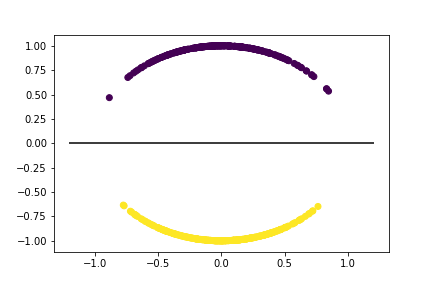
\includegraphics{feature-space.png} \\
        Figure 1: A depiction of feature space for the two clusters.
    \end{center}}
\end{document}